\chapter{Multiple Path Relay Network}
\label{chap:mp}

\begin{figure}
  \centering
    \psfrag{r0}[cc][Bl][0.9]{$r_0$}
    \psfrag{r1}[cc][Bl][0.9]{$r_1$}
    \psfrag{r3}[cc][Bl][0.9]{$r_m$}
    \psfrag{r4}[cc][Bl][0.9]{$r_{m+1}$}
    \psfrag{n01}[cc][Bl][0.8]{$n_k^{(0|1)}$}
    \psfrag{n03}[cc][Bl][0.8]{$n_k^{(0|m)}$}
    \psfrag{n14}[cc][Bl][0.8]{$n_k^{(1|m+1)}$}
    \psfrag{n34}[cc][Bl][0.8]{$n_k^{(m|m+1)}$}
    \psfrag{H01}[cc][Bl][0.8]{$h_k^{(0|1)}$}
    \psfrag{H03}[cc][Bl][0.8]{$h_k^{(0|m)}$}
    \psfrag{H14}[cc][Bl][0.8]{$h_k^{(1|m+1)}$}
    \psfrag{H34}[cc][Bl][0.8]{$h_k^{(m|m+1)}$}
    \psfrag{Tx}[cr][Bl][0.9]{Transmitter}
    \psfrag{Rx}[cl][Bl][0.9]{Receiver}
    \includegraphics[width=5in]{mp_model.eps}
   \caption{Multiple Path Relay Network \label{fig:mp_sm} }
\end{figure}

\section{Amplify-and-Forward}
\label{sec:mp_af}

\subsection{System Model}
\label{subsec:mp_af_sm}

Figure \ref{fig:mp_sm} shows the multiple path relay network.  In the figure, $r_0$ is the transmitter, $r_{m+1}$ is the receiver, and $r_1, \ldots, r_m$ are $m$ relay nodes connected in parallel forming a multiple path link between the transmitter and receiver.  The relays perform amplify-and-forward (AF) relaying.  We assume that OFDM with $N$ subcarriers is used in the system.

$h_k^{(0|1)}, \ldots, h_k^{(0|m)}, h_k^{(1|m+1)}, \ldots, h_k^{(m|m+1)}$ are the complex subchannel gains at the $k^{\mbox{th}}$ subcarrier in the link, for $k = 1$ to $N$.   $n_k^{(0|1)}, \ldots, n_k^{(0|m)}, n_k^{(1|m+1)}, \ldots, n_k^{(m|m+1)}$ are the corresponding noises, which are assumed to be mutually independent, zero-mean, circular symmetric complex Gaussians all with variance $N_0 B / N$, where $N_0$ is the power spectral density of the underlying continuous time noise process and $B$ is the OFDM bandwidth of the system.  Let $p_k^{(0)} = P_{\mbox{tot}}/N$ be the transmitter power on the $k^{\mbox{th}}$ subcarrier, where $P_{\mbox{tot}}$ is the net transmitter power.  Let  $\sqrt{p_k^{(l)}}$ be the amplifying gain used in the amplify-and-forward algorithm at the $l^{\mbox{th}}$ relay, for $l=1$ to $m$.  The $k^{\mbox{th}}$ receive symbol at $r_l$ is amplified by $\sqrt{p_k^{(l)}}$ before it is forwarded to the next node.

Let $x_k$ be the $k^{\mbox{th}}$ transmit symbol with zero mean and unit variance.  Let $y_k^{(l)}$  be the $k^{\mbox{th}}$ receive symbol from the $l^{\mbox{th}}$ path at the receiver.  Using Figure \ref{fig:mp_sm}, the input-output relation for the $l^{\mbox{th}}$ path is
\begin{eqnarray}
y_k^{(l)} = \left( h_k^{(0|l)} h_k^{(l|m+1)} \sqrt{p_k^{(0)}} \sqrt{p_k^{(l)}} \right) x_k
+\left( h_k^{(l|m+1)} \sqrt{p_k^{(l)}} \right) n_k^{(0|l)} +  n_k^{(l|m+1)}.
\label{eqn:mp_af_inout}
\end{eqnarray}
If we define
\begin{eqnarray}
\mathbf{y}_k = \left[
\begin{array}{ccc}
y_k^{(1)} &
\cdots &
y_k^{(m)} 
\end{array} \right]^T,
\end{eqnarray}
\begin{eqnarray}
\mathbf{h}_k = \left[
\begin{array}{ccc}
h_k^{(0|1)}h_k^{(1|m+1)} \sqrt{p_k^{(0)}} \sqrt{p_k^{(1)}} & \cdots & h_k^{(0|m)}h_k^{(m|m+1)} \sqrt{p_k^{(0)}} \sqrt{p_k^{(m)}}
\end{array}
\right]^T,
\label{eqn:mp_af_hk}
\end{eqnarray}
\begin{eqnarray}
\mathbf{\Gamma}_k = \left[
\begin{array}{cccccccc}
h_k^{(1|m+1)} \sqrt{p_k^{(1)}}&  & \textbf{\mbox{\huge{0}}} & 1 & & & & \textbf{\mbox{\huge{0}}}  \\
 & \ddots & & & & \ddots & &  \\
\textbf{\mbox{\huge{0}}} &  &h_k^{(m|m+1)} \sqrt{p_k^{(m)}} & \textbf{\mbox{\huge{0}}} & & & & 1 
\end{array}
\right]
\mbox{,}
\label{eqn:mp_af_Gammak}
\end{eqnarray}
\begin{eqnarray}
\mathbf{n}_k = \left[
\begin{array}{cccccc}
n_k^{(0|1)} & \cdots & n_k^{(0|m)} & n_k^{(1|m+1)} & \cdots & n_k^{(m|m+1)}
\end{array} \right]^T\mbox{,}
\label{eqn:mp_af_nk}
\end{eqnarray}
and
\begin{eqnarray}
\mathbf{w}_k = \mathbf{\Gamma}_k \mathbf{n}_k \mbox{,} 
\label{eqn:mp_af_wk}
\end{eqnarray}
then (\ref{eqn:mp_af_inout}), for all $l = 1$ to $m$, can be written as
\begin{eqnarray}
\mathbf{y}_k = \mathbf{h}_k x_k + \mathbf{w}_k \mbox{.}
\label{eqn:mp_af_inout_terse}
\end{eqnarray}
The large boldface zeros in (\ref{eqn:mp_af_Gammak}) represent zero values in the off diagonal entries in the two $m \times m$ submatrices of $\mathbf{\Gamma}_k$.  

Now, consider the covariance of $\mathbf{w}_k$.  Using (\ref{eqn:mp_af_Gammak}), (\ref{eqn:mp_af_nk}), and (\ref{eqn:mp_af_wk}), we have
\begin{eqnarray}
R_{\mathbf{w}_k\mathbf{w}_k} & = & E \left[ \mathbf{w}_k \mathbf{w}_k^H \right] \\
& = & E \left[ \mathbf{\Gamma}_k \mathbf{n}_k \mathbf{n}_k^H \mathbf{\Gamma}_k^H \right] \\
& = & \mathbf{\Gamma}_k E \left[ \mathbf{n}_k \mathbf{n}_k^H  \right] \mathbf{\Gamma}_k^H \\
& = &  \frac{N_0B}{N} \left[
\begin{array}{ccc}
b_k^{(1|m+1)} p_k^{(1)}  + 1 & & \textbf{\mbox{\huge{0}}} \\
 & \ddots & \\
\textbf{\mbox{\huge{0}}}  & &  b_k^{(m|m+1)} p_k^{(m)} + 1
\end{array} \right],
\label{eqn:mp_af_Rwkwk}
\end{eqnarray}
where $E\left[ \cdot \right]$ is the expectation operator, $\left( \cdot \right)^H$ is the Hermitian (complex transpose) operator for a vector or matrix, and $b_k^{(i|j)} = \left| h_k^{(i|j)} \right|^2$, for $i=0$ to $m$, for $j=1$ to $m+1$, and $i \neq j$.  Since the diagonal entries of $R_{\mathbf{w}_k\mathbf{w}_k}$ are never zero, $R_{\mathbf{w}_k\mathbf{w}_k}^{-1}$ and $R_{\mathbf{w}_k\mathbf{w}_k}^{-\frac{1}{2}}$ are well defined, where $R_{\mathbf{w}_k\mathbf{w}_k}^{-\frac{1}{2}}R_{\mathbf{w}_k\mathbf{w}_k}^{-\frac{1}{2}} = R_{\mathbf{w}_k\mathbf{w}_k}^{-1}$
\begin{eqnarray}
R_{\mathbf{w}_k\mathbf{w}_k}^{-1} = \frac{N}{N_0B} \left[
\begin{array}{ccc}
\frac{1}{ b_k^{(1|m+1)} p_k^{(1)}+ 1} & & \textbf{\mbox{\huge{0}}} \\
 & \ddots & \\
\textbf{\mbox{\huge{0}}}  & & \frac{1}{ b_k^{(m|m+1)}p_k^{(m)} + 1}
.\label{eqn:mp_af_Rwkwk_inv}
\end{array} \right]. 
\end{eqnarray}
Also, if we define $R_{\mathbf{w}_k\mathbf{w}_k}$ as $R_{\mathbf{w}_k\mathbf{w}_k}^{\frac{1}{2}} R_{\mathbf{w}_k\mathbf{w}_k}^{\frac{1}{2}} =R_{\mathbf{w}_k\mathbf{w}_k}$, then $R_{\mathbf{w}_k\mathbf{w}_k}^{-\frac{1}{2}}R_{\mathbf{w}_k\mathbf{w}_k}^{\frac{1}{2}} = R_{\mathbf{w}_k\mathbf{w}_k}^{\frac{1}{2}}R_{\mathbf{w}_k\mathbf{w}_k}^{-\frac{1}{2}} = \mathbf{I}$.
We define a transformed version of the system in (\ref{eqn:mp_af_inout_terse})
\begin{eqnarray}
\tilde{\mathbf{y}}_k = \tilde{\mathbf{h}}_k x_k + \tilde{\mathbf{w}}_k,
\end{eqnarray}
where $\tilde{\mathbf{y}}_k = R_{\mathbf{w}_k\mathbf{w}_k}^{-\frac{1}{2}} \mathbf{y}_k$, $\tilde{\mathbf{h}}_k =R_{\mathbf{w}_k\mathbf{w}_k}^{-\frac{1}{2}} \mathbf{h}_k$, and $\tilde{\mathbf{w}}_k = R_{\mathbf{w}_k\mathbf{w}_k}^{-\frac{1}{2}} \mathbf{w}_k$.  The covariance matrices of $\tilde{\mathbf{w}}_k$ and $\tilde{\mathbf{y}}_k$ are
\begin{eqnarray}
E \left[ \tilde{\mathbf{w}}_k \tilde{\mathbf{w}}_k^H \right] & = & E \left[R_{\mathbf{w}_k\mathbf{w}_k}^{-\frac{1}{2}} \mathbf{w}_k \mathbf{w}_k^H R_{\mathbf{w}_k\mathbf{w}_k}^{-\frac{1}{2}} \right] \\
& = & R_{\mathbf{w}_k\mathbf{w}_k}^{-\frac{1}{2}} R_{\mathbf{w}_k\mathbf{w}_k}R_{\mathbf{w}_k\mathbf{w}_k}^{-\frac{1}{2}} \\
& = & \mathbf{I} 
\end{eqnarray}
and
\begin{eqnarray}
E \left[ \tilde{\mathbf{y}}_k \tilde{\mathbf{y}}_k^H \right] & = & E \left[ \left(\tilde{\mathbf{h}_k}x_k + \tilde{\mathbf{w}_k}\right) \left(\tilde{\mathbf{h}_k}x_k + \tilde{\mathbf{w}_k}\right)^H \right] 
\\
& = & \tilde{\mathbf{h}}_k \tilde{\mathbf{h}}_k^H + \mathbf{I},
\label{eqn:mp_af_yk_tilde_covar}
\end{eqnarray}
respectively.  The cross terms do not appear in (\ref{eqn:mp_af_yk_tilde_covar}) because $\tilde{\mathbf{h}_k}$, $\tilde{\mathbf{w}_k}$ and $x_k$ are mutually independent.  Note that the transformed system has identity covariance noise.

\subsection{Mutual Information}
\label{subsec:mp_af_mi}

To derive the mutual information, note that the differential entropy of a circular symmetric complex Gaussian vector, $\mathbf{v}$, with covariance matrix, $\mathbf{K}$, is $h\left(\mathbf{v}\right) = \log_2 \det \left( \pi e \mathbf{K} \right)$ \cite{article:Telatar01}.  Let $\mathcal{I}_k$ be the mutual information between the transmitter and receiver on the $k^{\mbox{th}}$ subcarrier
\begin{eqnarray}
\mathcal{I}_k & = & h\left( \tilde{\mathbf{y}}_k \right) - h \left( \tilde{\mathbf{w}}_k \right)  \\
& = & \log_2 \det\left[ \pi e \left(\tilde{\mathbf{h}}_k \tilde{\mathbf{h}}_k^H + \mathbf{I} \right) \right] 
- \log_2 \det \left( \pi e \mathbf{I} \right)  \\
& = & \log_2 \left( 1 + \mathbf{h}_k^H R_{\mathbf{w}_k\mathbf{w}_k}^{-1} \mathbf{h}_k \right),
\label{eqn:mp_af_Ik}
\end{eqnarray}
where the first equality comes from basic mutual information calculations \cite{book:Cover01}.  The third equality follows from the properties of determinants of matrices.  The total mutual information between the transmitter and receiver, $\mathcal{I}$, is the sum of all $\mathcal{I}_k$ divided by $N$.  That is, after substituting (\ref{eqn:mp_af_hk}) and (\ref{eqn:mp_af_Rwkwk_inv}) into (\ref{eqn:mp_af_Ik}), we have
\begin{eqnarray}
\mathcal{I} & = & \frac{1}{N}  \sum_{k=1}^N \mathcal{I}_k \\
& = & \frac{1}{N}  \sum_{k=1}^N \log_2 \left[ 1 + \mbox{SNR} \sum_{i=1}^m \left(
\frac{b_k^{(0|i)} b_k^{(i|m+1)}p_k^{(i)}  }{ b_k^{(i|m+1)} p_k^{(i)}+1 }\right) \right],
\label{eqn:mp_af_I}
\end{eqnarray}
where $\mbox{SNR} = P_{\mbox{tot}}/N_0B$.  If we denote	
\begin{eqnarray}
\mathbf{B}^{(\mbox{sr})} = \left[ \begin{array}{ccc}
b_1^{(0|1)} & \cdots & b_1^{(0|m)} \\
\vdots & \ddots & \vdots \\
b_N^{(0|1)} & \cdots & b_N^{(0|m)}
\end{array}
\right] \mbox{,} &
\mathbf{B}^{(\mbox{rd})} = \left[ \begin{array}{ccc}
b_1^{(1|m+1)} & \cdots & b_1^{(m|m+1)} \\
\vdots & \ddots & \vdots \\
b_N^{(1|m+1)} & \cdots & b_N^{(m|m+1)}
\end{array}
\right] \mbox{,}
\label{}
\end{eqnarray}
\begin{eqnarray}
 & \mathbf{P} = \left[ \begin{array}{ccc}
p_1^{(1)} & \cdots & p_1^{(m)} \\
\vdots & \ddots & \vdots \\
p_N^{(1)} & \cdots & p_N^{(m)}
\end{array}
\right] \mbox{,}
\label{}
\end{eqnarray}
\begin{eqnarray}
\begin{array}{ccc}
\mathbf{e}_N = \underbrace{\left[ \begin{array}{ccc}
1 & \cdots & 1
\end{array}
\right]^T}_{\mbox{$N$ ones}} \mbox{,}& \mbox{and} &
\mathbf{e}_m = \underbrace{\left[ \begin{array}{ccc}
1 & \cdots & 1
\end{array}
\right]^T}_{\mbox{$m$ ones}},
\end{array}
\label{}
\end{eqnarray}
then (\ref{eqn:mp_af_I}) can be written in matrix form.  First, let
\begin{eqnarray}
\mathbf{z}_{\mbox{multiple}} = 
\left[ \left( \mathbf{B}^{(\mbox{sr})} \circ \mathbf{B}^{(\mbox{rd})} \circ \mathbf{P}  \right) \circ / \left( \mathbf{B}^{(\mbox{rd})} \circ \mathbf{P}  + \mathbf{e}_N \mathbf{e}_m^T \right) \right] \mathbf{e}_m,
\end{eqnarray}
where the $\circ$ and $\circ /$ operators represent element-wise matrix multiplication and element-wise matrix division, respectively.  Then, (\ref{eqn:mp_af_I}) in matrix form is
\begin{eqnarray}
\mathcal{I} = \frac{1}{N} \mathbf{e}_N^T \log_2 \left( \mathbf{e}_N + \mbox{SNR} \: \mathbf{z}_{\mbox{multiple}} \right) ,
\label{eqn:mp_af_I_matrix}
\end{eqnarray}
where $\log_2\left( \cdot \right)$ of a vector is the vector of the logarithms of the vector's entries.

\subsection{Relay Power Allocation}
\label{subsec:mp_af_rpa}

We assume that the net transmit power at the transmitter and at each each relay is $P_{\mbox{tot}}$.  At the transmitter, we assume a uniform power distribution, that is, $p_k^{(0)} = P_{\mbox{tot}}/N$.  To derive the power constraint at each relay and thus, possible power allocations, consider $v_k^{(l)}$, the $k^{\mbox{th}}$ transmit symbol of $r_l$
\begin{eqnarray}
v_k^{(l)} = \sqrt{p_k^{(l)}} \left[ \left(  h_k^{(0|l)}  \sqrt{p_k^{(0)}} \right)  x_k + n_k^{(0|l)} \right] \mbox{.}
\end{eqnarray}
The constraint is $P_{\mbox{tot}} = \displaystyle \sum_{k=1}^{N} E \left[ \left| v_k^{(l)} \right|^2 \right]$.  Thus,
\begin{eqnarray}
P_{\mbox{tot}} = \displaystyle \sum_{k=1}^{N} p_k^{(l)}
\left( b_k^{(0|l)} \frac{P_{\mbox{tot}}}{N}  + 
\frac{N_0 B}{N} \right)
\label{eqn:mp_af_powerconstraint0}
\end{eqnarray}
or
\begin{eqnarray}
\sum_{k=1}^N \frac{ p_k^{(l)}}{N} \left(
b_k^{(0|l)} + 
\frac{1}{\mbox{SNR}} \right) =1.
\label{eqn:mp_af_powerconstraint}
\end{eqnarray}

One power allocation at the $l^{\mbox{th}}$ relay is to set $p_k^{(l)}$ constant for all subcarriers.  This results in moving $p_k^{(l)}$ in (\ref{eqn:mp_af_powerconstraint}) out of the summation because it is no longer a function of $k$
\begin{eqnarray}
p_{k,ct}^{(l)} = p_{ct}^{(l)} = 
 \frac{N \mbox{SNR}}
{\displaystyle \sum_{k=1}^N \left( \mbox{SNR} b_k^{(0)} + 1 \right)
} \mbox{.}
\end{eqnarray}
We call this \emph{constant gain allocation} (CT).  Note that this power allocation does not require each relay to have any CSI (channel state information).  The $l^{\mbox{th}}$ relay only has to multiply its entire OFDM receive symbol by a constant, $\sqrt{p_{ct}^{(l)}}$, such that the total transmit power is $P_{\mbox{tot}}$.  We call \emph{constant 
gain capacity}, $C_{ct}$, as the mutual information in (\ref{eqn:mp_af_I_matrix}) resulting from this power allocation.

A second power allocation is to choose $p_k^{(l)}$ such that every subcarrier transmits the same power at the $l^{\mbox{th}}$ relay.  The transmit power on the $k^{\mbox{th}}$ subcarrier is the $k^{\mbox{th}}$ summand on the right hand side of (\ref{eqn:mp_af_powerconstraint0}).  Since they are all equal to $P_{\mbox{tot}}/N$, we have
\begin{eqnarray}
\frac{P_{\mbox{tot}}}{N} = 
 p_{k,eq}^{(l)}
\left( b_k^{(0|l)} \frac{P_{\mbox{tot}}}{N}   + 
\frac{N_0 B}{N}
\right) \end{eqnarray}
or
\begin{eqnarray}
p_{k,eq}^{(l)} =  \frac{ \mbox{SNR}}
{\displaystyle  \mbox{SNR} b_k^{(0|l)} + 1} \mbox{.}
\end{eqnarray}
We call this \emph{equal power allocation} (EQ).  Note that this power allocation does require each relay to have the CSI of its upstream channel.  We call \emph{equal power capacity}, $C_{eq}$, as the mutual information in (\ref{eqn:mp_af_I_matrix}) resulting from this power allocation.

\subsection{Capacity Simulations}
\label{subsec:mp_af_cs}

We simulate $C_{ct}$ and $C_{eq}$ assuming that all distances between any two adjacent transceiver nodes are the same.  Therefore, all path loss effects are normalized to $0$ dB.  Shadowing between nodes is assumed to be log-normally distributed.  That is, the received power gain due to shadowing in dB is a zero-mean Gaussian with variance of 8 dB, which is typical for cellular land mobile applications \cite{book:Stuber01}.  We model frequency selective fading effects as Typical Urban (TU) channels and Hilly Terrain (HT) channels \cite{book:Stuber01}.  We use an OFDM bandwidth of 800 kHz divided into $N=128$ equal blocks.  Maintaining OFDM orthogonality, this translates into an OFDM symbol period of $T_s = 160\:\mu$s.  Results are shown in Figures \ref{fig:mp_af_cap_plots_TU} and \ref{fig:mp_af_cap_plots_HT}.

The plots exhibit the familiar monotonically increasing shape for mutual information in the case of direct transmission between a transmitter and receiver.  This is expected if we look at the mutual information in (\ref{eqn:mp_af_I_matrix}).  We can think of this configuration as still being direct transmission where the channel is the single path relay network, characterized by $\mathbf{z}_{\mbox{multiple}}$.  Note that $\mathbf{z}_{\mbox{multiple}}$ also determines the power allocations in the relays.  In other words, (\ref{eqn:mp_af_I_matrix}) is a system level representation of the mutual information.

As we increase the number of paths between the transmitter and receiver (and thus, add more relays), more noise and channel distortion enter the system.  However, adding more paths increases the throughput of the system.  Consequently, the net result is that the mutual information increases.  Constant gain allocation and equal power allocation are practically the same.  TU channels and HT channels give very similar results.


\begin{figure*}
    \psfrag{Capacity}[Bc][tc][0.8]{Capacity (bits/s/Hz)}
    \psfrag{SNR}[tc][Bc][0.8]{SNR (dB)}
    \psfrag{Cct-}[cl][cl][0.6]{$C_{ct}$}
    \psfrag{Ceq-}[cl][cl][0.6]{$C_{eq}$}
    \psfrag{Caa-}[cl][cl][0.6]{$C_{aa}$}
\centerline{
	\subfigure[m=1]{\includegraphics[width=3in]{mp_af_cap_m1_TU.eps} \label{}} 
	\subfigure[m=2]{\includegraphics[width=3in]{mp_af_cap_m2_TU.eps} \label{}} \\
}
\centerline{
	\subfigure[m=3]{\includegraphics[width=3in]{mp_af_cap_m3_TU.eps} \label{}}
	\subfigure[m=4]{\includegraphics[width=3in]{mp_af_cap_m4_TU.eps} \label{}} \\
}
\caption{Capacity in a multiple path relay network with TU channels using AF.  $N = 128, m = 1, 2, 3$, and $4$.}
\label{fig:mp_af_cap_plots_TU}
\end{figure*}

\begin{figure*}
    \psfrag{Capacity}[Bc][tc][0.8]{Capacity (bits/s/Hz)}
    \psfrag{SNR}[tc][Bc][0.8]{SNR (dB)}
    \psfrag{Cct-}[cl][cl][0.6]{$C_{ct}$}
    \psfrag{Ceq-}[cl][cl][0.6]{$C_{eq}$}
    \psfrag{Caa-}[cl][cl][0.6]{$C_{aa}$}
\centerline{
	\subfigure[m=1]{\includegraphics[width=3in]{mp_af_cap_m1_HT.eps} \label{}} 
	\subfigure[m=2]{\includegraphics[width=3in]{mp_af_cap_m2_HT.eps} \label{}} \\
}
\centerline{
	\subfigure[m=3]{\includegraphics[width=3in]{mp_af_cap_m3_HT.eps} \label{}}
	\subfigure[m=4]{\includegraphics[width=3in]{mp_af_cap_m4_HT.eps} \label{}} \\
}
\caption{Capacity in a multiple path relay network with HT channels using AF.  $N = 128, m = 1, 2, 3$, and $4$.}
\label{fig:mp_af_cap_plots_HT}
\end{figure*}


\section{Decode-and-Forward}
\label{sec:mp_df}

\subsection{System Model}
\label{subsec:mp_df_sm}

In decode-and-forward (DF), each relay fully recovers the information bits (with possible errors) after receiving an OFDM symbol.  It then converts the information bits back into an OFDM symbol and then transmits it.  The transmitter and all the relays transmit with the same uniform power distribution.  That is,
\begin{eqnarray}
p_k^{(0)} = p_k^{(l)} = \frac{P_{\mbox{tot}}}{N}\mbox{,}
\end{eqnarray}
for $k = 1$ to $N$ and for $l = 1$ to $m$.

Let $x_k^{(0)}$ be the $k^{\mbox{th}}$ transmit symbol from the transmitter and  $x_k^{(l)}$ be the $k^{\mbox{th}}$ transmit symbol from the $l^{\mbox{th}}$ relay, all with with zero mean and unit variance.  Let $y_k^{(m+1)}$ be the $k^{\mbox{th}}$ receive symbol at the receiver and  $y_k^{(l)}$ be the $k^{\mbox{th}}$ receive symbol at the $l^{\mbox{th}}$ relay.  Using Figure \ref{fig:mp_sm}, the input-ouput relation at the $l^{\mbox{th}}$ relay is
\begin{eqnarray}
y_k^{(l)} = h_k^{(0|l)} \sqrt{\frac{P_{\mbox{tot}}}{N}} x_k^{(0)} + n_k^{(0|l)} \mbox{.}
\end{eqnarray}
The input-output relation at the receiver is
\begin{eqnarray}
y_k^{(m+1)} = \sum_{i=1}^m\left( h_k^{(i|m+1)}  \sqrt{\frac{P_{\mbox{tot}}}{N}} x_k^{(i)} + n_k^{(i|m+1)} \right)\mbox{.}
\end{eqnarray}
Note that in this situation, there are $m$ (modified in general) copies of the original $k^{\mbox{th}}$ transmit symbol $x_k^{(0)}$, namely, $x_k^{(1)}, \ldots, x_k^{(m)}$.  Therefore, the receiver has to assume (incorrectly in general) that all $m$ relays perform perfect recovery of the information bits so that $x_k^{(l)}$ = $x_k^{(0)}$.  That is, the receiver assumes the $k^{\mbox{th}}$ receive symbol is
\begin{eqnarray}
y_k^{(m)} = \left( \sum_{i=1}^m h_k^{(i|m+1)}  \sqrt{\frac{P_{\mbox{tot}}}{N}} \right) x_k^{(0)} + \sum_{i=1}^m n_k^{(i|m+1)} \mbox{.}
\end{eqnarray}
This allows the receiver to use a filter that is matched to $\displaystyle \sum_{i=1}^m h_k^{(i|m+1)}$.

\section{BER and WER Simulations}
\label{sec:mp_bws}

We simulate bit error rates (BERs) and word error rates (WERs) for both the amplify-and-forward and decode-and-forward cases.  At the transmitter (and at the transmitter structure of a relay using decode-and-forward), each information word contains 83 bits.  Using the convolutional encoder shown in Figure \ref{fig:conv_enc}, the information word is encoded into a 255 bit codeword.  A zero bit is padded at the end to make 256 bits.  The bits are then interleaved and modulated onto $N = 128$ QPSK (quadrature phase shift keying) subcarriers to form one OFDM symbol.  At the receiver (and at the receiver structure of a relay using decode-and-forward), the codeword is recovered (with possible errors) using a matched filter and deinterleaving.  A Viterbi decoder is used to decode the codeword.  Both hard decisions and soft decisions are used.

We assume that all distances between any two adjacent transceiver nodes are the same.  Therefore, all path loss effects are normalized to 0 dB.  Shadowing is assumed to be log-normally distributed.  That is, the received power gain due to shadowing in dB is a zero-mean Gaussian with variance of 8 dB, which is typical for cellular land mobile applications \cite{book:Stuber01}.  We model frequency selective fading as Typical Urban (TU) channels and Hilly Terrain (HT) channels \cite{book:Stuber01}.  We use an OFDM bandwidth of 800 kHz divided into $N = 128$ equal blocks.  Maintaining OFDM orthogonality, this translates into an OFDM symbol period of $T_s = 160 \:\mu$s.  

\subsection{Amplify-and-Forward}
\label{subsec:mp_bws_af}

The BER versus SNR and WER versus SNR plots for a single path relay network with TU channels using amplify-and-forward are shown in Figures \ref{fig:mp_af_ber_plots_TU} and \ref{fig:mp_af_wer_plots_TU}, respectively.  The corresponding plots for HT channels are shown in Figures \ref{fig:mp_af_ber_plots_HT} and \ref{fig:mp_af_wer_plots_HT}, respectively.

As expected, soft decisions in Viterbi decoding give better performance than hard decisions.  In particular, there is up to 4 dB of SNR gain.  In general, using hard decisions with equal power allocation results in the worst performance, except for the $m=1$ case, where hard decisions with constant allocation is the worst.  Soft decisions with constant gain allocation gives the best performance.

As we increase the number of paths between the transmitter and receiver (and thus, add more relays), the throughput of the system increases.  As a result, the error rate (BER and WER) performance improves, as shown in the plots.  TU channels and HT channels give very similar results.

\begin{figure*}
    \psfrag{BER}[Bc][tc][0.8]{BER}
    \psfrag{SNR}[tc][Bc][0.8]{SNR (dB)}
    \psfrag{hard--constant-gain-allocation}[cl][cl][0.5]{hard, constant gain allocation}
    \psfrag{hard--equal-power-allocation}[cl][cl][0.5]{hard, equal power allocation}
    \psfrag{soft--constant-gain-allocation}[cl][cl][0.5]{soft, constant gain allocation}
    \psfrag{soft--equal-power-allocation}[cl][cl][0.5]{soft, equal power allocation}

\centerline{
	\subfigure[m=1]{\includegraphics[width=3in]{mp_af_ber_m1_TU.eps} \label{}} 
	\subfigure[m=2]{\includegraphics[width=3in]{mp_af_ber_m2_TU.eps} \label{}} \\
}
\centerline{
	\subfigure[m=3]{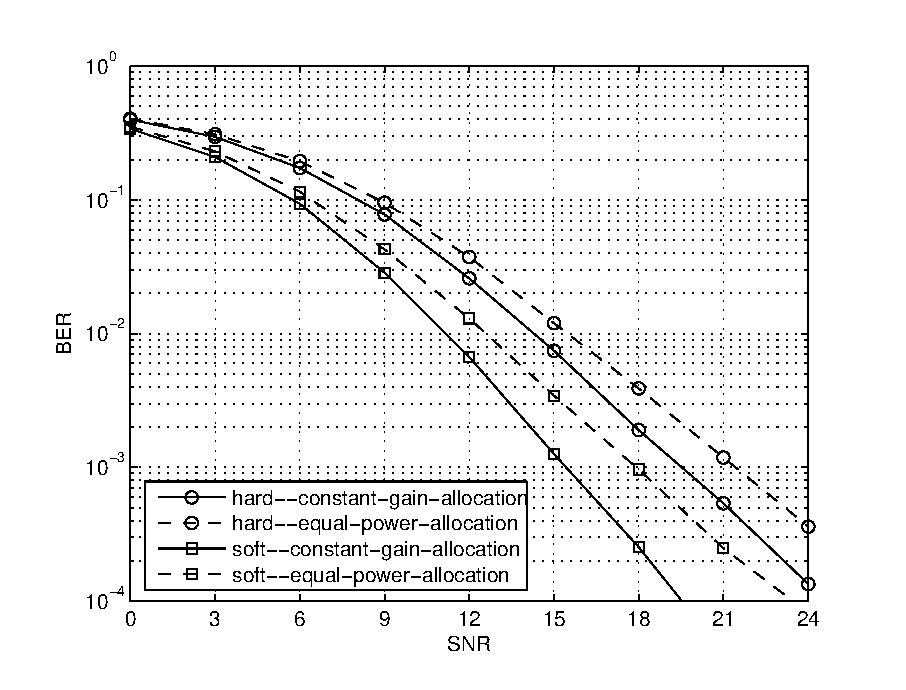
\includegraphics[width=3in]{mp_af_ber_m3_TU.eps} \label{}}
	\subfigure[m=4]{\includegraphics[width=3in]{mp_af_ber_m4_TU.eps} \label{}} \\
}
\caption{BER in a multiple path relay network with TU channels using AF.  $N = 128, m = 1, 2, 3$, and $4$.}
\label{fig:mp_af_ber_plots_TU}
\end{figure*}

\begin{figure*}
    \psfrag{WER}[Bc][tc][0.8]{WER}
    \psfrag{SNR}[tc][Bc][0.8]{SNR (dB)}
    \psfrag{hard--constant-gain-allocation}[cl][cl][0.5]{hard, constant gain allocation}
    \psfrag{hard--equal-power-allocation}[cl][cl][0.5]{hard, equal power allocation}
    \psfrag{soft--constant-gain-allocation}[cl][cl][0.5]{soft, constant gain allocation}
    \psfrag{soft--equal-power-allocation}[cl][cl][0.5]{soft, equal power allocation}

\centerline{
	\subfigure[m=1]{\includegraphics[width=3in]{mp_af_wer_m1_TU.eps} \label{}} 
	\subfigure[m=2]{\includegraphics[width=3in]{mp_af_wer_m2_TU.eps} \label{}} \\
}
\centerline{
	\subfigure[m=3]{\includegraphics[width=3in]{mp_af_wer_m3_TU.eps} \label{}}
	\subfigure[m=4]{\includegraphics[width=3in]{mp_af_wer_m4_TU.eps} \label{}} \\
}
\caption{WER in a multiple path relay network with TU channels using AF.  $N = 128, m = 1, 2, 3$, and $4$.}
\label{fig:mp_af_wer_plots_TU}
\end{figure*}

\begin{figure*}
    \psfrag{BER}[Bc][tc][0.8]{BER}
    \psfrag{SNR}[tc][Bc][0.8]{SNR (dB)}
    \psfrag{hard--constant-gain-allocation}[cl][cl][0.5]{hard, constant gain allocation}
    \psfrag{hard--equal-power-allocation}[cl][cl][0.5]{hard, equal power allocation}
    \psfrag{soft--constant-gain-allocation}[cl][cl][0.5]{soft, constant gain allocation}
    \psfrag{soft--equal-power-allocation}[cl][cl][0.5]{soft, equal power allocation}

\centerline{
	\subfigure[m=1]{\includegraphics[width=3in]{mp_af_ber_m1_HT.eps} \label{}} 
	\subfigure[m=2]{\includegraphics[width=3in]{mp_af_ber_m2_HT.eps} \label{}} \\
}
\centerline{
	\subfigure[m=3]{\includegraphics[width=3in]{mp_af_ber_m3_HT.eps} \label{}}
	\subfigure[m=4]{\includegraphics[width=3in]{mp_af_ber_m4_HT.eps} \label{}} \\
}
\caption{BER in a multiple path relay network with HT channels using AF.  $N = 128, m = 1, 2, 3$, and $4$.}
\label{fig:mp_af_ber_plots_HT}
\end{figure*}

\begin{figure*}
    \psfrag{WER}[Bc][tc][0.8]{WER}
    \psfrag{SNR}[tc][Bc][0.8]{SNR (dB)}
    \psfrag{hard--constant-gain-allocation}[cl][cl][0.5]{hard, constant gain allocation}
    \psfrag{hard--equal-power-allocation}[cl][cl][0.5]{hard, equal power allocation}
    \psfrag{soft--constant-gain-allocation}[cl][cl][0.5]{soft, constant gain allocation}
    \psfrag{soft--equal-power-allocation}[cl][cl][0.5]{soft, equal power allocation}

\centerline{
	\subfigure[m=1]{\includegraphics[width=3in]{mp_af_wer_m1_HT.eps} \label{}} 
	\subfigure[m=2]{\includegraphics[width=3in]{mp_af_wer_m2_HT.eps} \label{}} \\
}
\centerline{
	\subfigure[m=3]{\includegraphics[width=3in]{mp_af_wer_m3_HT.eps} \label{}}
	\subfigure[m=4]{\includegraphics[width=3in]{mp_af_wer_m4_HT.eps} \label{}} \\
}
\caption{WER in a multiple path relay network with HT channels using AF.  $N = 128, m = 1, 2, 3$, and $4$.}
\label{fig:mp_af_wer_plots_HT}
\end{figure*}

\subsection{Decode-and-Forward}
\label{subsec:mp_bws_df}

The BER versus SNR and WER versus SNR plots for a single path relay network with TU channels using decode-and-forward are shown in Figures \ref{fig:mp_df_ber_plots_TU} and \ref{fig:mp_df_wer_plots_TU}, respectively.  The corresponding plots for HT channels are shown in Figures \ref{fig:mp_df_ber_plots_HT} and \ref{fig:mp_df_wer_plots_HT}, respectively.

As expected, soft decisions in Viterbi decoding give better performance than hard decisions.  In particular, there is up to 5 dB of SNR gain, as shown in the plots.

As we increase the number of paths between the transmitter and receiver (and thus, add more relays), the error rate (BER and WER) performance remains largely the same, as shown in the plots.  TU channels and HT channels give very similar results.



\begin{figure*}
    \psfrag{BER}[Bc][tc][0.8]{BER}
    \psfrag{SNR}[tc][Bc][0.8]{SNR (dB)}
    \psfrag{hard}[cl][cl][0.5]{hard}
    \psfrag{soft}[cl][cl][0.5]{soft}

\centerline{
	\subfigure[m=1]{\includegraphics[width=3in]{mp_df_ber_m1_TU.eps} \label{}} 
	\subfigure[m=2]{\includegraphics[width=3in]{mp_df_ber_m2_TU.eps} \label{}} \\
}
\centerline{
	\subfigure[m=3]{\includegraphics[width=3in]{mp_df_ber_m3_TU.eps} \label{}}
	\subfigure[m=4]{\includegraphics[width=3in]{mp_df_ber_m4_TU.eps} \label{}} \\
}
\caption{BER in a multiple path relay network with TU channels using DF.  $N = 128, m = 1, 2, 3$, and $4$.}
\label{fig:mp_df_ber_plots_TU}
\end{figure*}

\begin{figure*}
    \psfrag{WER}[Bc][tc][0.8]{WER}
    \psfrag{SNR}[tc][Bc][0.8]{SNR (dB)}
    \psfrag{hard}[cl][cl][0.5]{hard}
    \psfrag{soft}[cl][cl][0.5]{soft}

\centerline{
	\subfigure[m=1]{\includegraphics[width=3in]{mp_df_wer_m1_TU.eps} \label{}} 
	\subfigure[m=2]{\includegraphics[width=3in]{mp_df_wer_m2_TU.eps} \label{}} \\
}
\centerline{
	\subfigure[m=3]{\includegraphics[width=3in]{mp_df_wer_m3_TU.eps} \label{}}
	\subfigure[m=4]{\includegraphics[width=3in]{mp_df_wer_m4_TU.eps} \label{}} \\
}
\caption{WER in a multiple path relay network with TU channels using DF.  $N = 128, m = 1, 2, 3$, and $4$.}
\label{fig:mp_df_wer_plots_TU}
\end{figure*}

\begin{figure*}
    \psfrag{BER}[Bc][tc][0.8]{BER}
    \psfrag{SNR}[tc][Bc][0.8]{SNR (dB)}
    \psfrag{hard}[cl][cl][0.5]{hard}
    \psfrag{soft}[cl][cl][0.5]{soft}

\centerline{
	\subfigure[m=1]{\includegraphics[width=3in]{mp_df_ber_m1_HT.eps} \label{}} 
	\subfigure[m=2]{\includegraphics[width=3in]{mp_df_ber_m2_HT.eps} \label{}} \\
}
\centerline{
	\subfigure[m=3]{\includegraphics[width=3in]{mp_df_ber_m3_HT.eps} \label{}}
	\subfigure[m=4]{\includegraphics[width=3in]{mp_df_ber_m4_HT.eps} \label{}} \\
}
\caption{BER in a multiple path relay network with HT channels using DF.  $N = 128, m = 1, 2, 3$, and $4$.}
\label{fig:mp_df_ber_plots_HT}
\end{figure*}

\begin{figure*}
    \psfrag{WER}[Bc][tc][0.8]{WER}
    \psfrag{SNR}[tc][Bc][0.8]{SNR (dB)}
    \psfrag{hard}[cl][cl][0.5]{hard}
    \psfrag{soft}[cl][cl][0.5]{soft}

\centerline{
	\subfigure[m=1]{\includegraphics[width=3in]{mp_df_wer_m1_HT.eps} \label{}} 
	\subfigure[m=2]{\includegraphics[width=3in]{mp_df_wer_m2_HT.eps} \label{}} \\
}
\centerline{
	\subfigure[m=3]{\includegraphics[width=3in]{mp_df_wer_m3_HT.eps} \label{}}
	\subfigure[m=4]{\includegraphics[width=3in]{mp_df_wer_m4_HT.eps} \label{}} \\
}
\caption{WER in a multiple path relay network with HT channels using DF.  $N = 128, m = 1, 2, 3$, and $4$.}
\label{fig:mp_df_wer_plots_HT}
\end{figure*}

\subsection{Comparison}
\label{subsec:mp_bws_c}

The BER versus SNR and WER versus SNR plots for a multiple path relay network with TU channels using amplify-and-forward and decode-and-forward are shown in Figures \ref{fig:mp_af_df_ber_plots_TU} and \ref{fig:mp_af_df_wer_plots_TU}, respectively.  The corresponding plots for HT channels are shown in Figures \ref{fig:mp_af_df_ber_plots_HT} and \ref{fig:mp_af_df_wer_plots_HT}, respectively.

When $m=1$, using decode-and-forward with soft decisions provides an SNR performance gain of 3 dB over the best amplify-and-forward scheme.  However, as we increase the number of paths between the transmitter and receiver (and thus, add more relays), the performance gains resulting from using decode-and-forward instead of amplify-and-forward diminish, as shown in Figures \ref{fig:mp_af_df_ber_m4_TU}, \ref{fig:mp_af_df_wer_m4_TU}, \ref{fig:mp_af_df_ber_m4_HT}, and \ref{fig:mp_af_df_wer_m4_HT}.  This is because for $m=4$ relays and thus, for 4 paths, the system is already resistant to noise and channel distortion.  Therefore, decode-and-forward cannot provide any more significant improvement over amplify-and-forward.

\begin{figure*}
    \psfrag{BER}[Bc][tc][0.8]{BER}
    \psfrag{SNR}[tc][Bc][0.8]{SNR (dB)}
    \psfrag{hard-af-ct----}[cl][cl][0.5]{hard, AF, CT}
    \psfrag{hard-af-eq----}[cl][cl][0.5]{hard, AF, EQ}
    \psfrag{hard-df----}[cl][cl][0.5]{hard, DF}
    \psfrag{soft-af-ct----}[cl][cl][0.5]{soft, AF, CT}
    \psfrag{soft-af-eq----}[cl][cl][0.5]{soft, AF, EQ}
    \psfrag{soft-df----}[cl][cl][0.5]{soft, DF}

\centerline{
	\subfigure[m=1]{\includegraphics[width=3in]{mp_af_df_ber_m1_TU.eps} \label{}} 
	\subfigure[m=2]{\includegraphics[width=3in]{mp_af_df_ber_m2_TU.eps} \label{}} \\
}
\centerline{
	\subfigure[m=3]{\includegraphics[width=3in]{mp_af_df_ber_m3_TU.eps} \label{}}
	\subfigure[m=4]{\includegraphics[width=3in]{mp_af_df_ber_m4_TU.eps} \label{fig:mp_af_df_ber_m4_TU}} \\
}
\caption{BER in a multiple path relay network with TU channels using AF and DF.  $N = 128, m = 1, 2, 3$, and $4$.}
\label{fig:mp_af_df_ber_plots_TU}
\end{figure*}

\begin{figure*}
    \psfrag{WER}[Bc][tc][0.8]{WER}
    \psfrag{SNR}[tc][Bc][0.8]{SNR (dB)}
    \psfrag{hard-af-ct----}[cl][cl][0.5]{hard, AF, CT}
    \psfrag{hard-af-eq----}[cl][cl][0.5]{hard, AF, EQ}
    \psfrag{hard-df----}[cl][cl][0.5]{hard, DF}
    \psfrag{soft-af-ct----}[cl][cl][0.5]{soft, AF, CT}
    \psfrag{soft-af-eq----}[cl][cl][0.5]{soft, AF, EQ}
    \psfrag{soft-df----}[cl][cl][0.5]{soft, DF}

\centerline{
	\subfigure[m=1]{\includegraphics[width=3in]{mp_af_df_wer_m1_TU.eps} \label{}} 
	\subfigure[m=2]{\includegraphics[width=3in]{mp_af_df_wer_m2_TU.eps} \label{}} \\
}
\centerline{
	\subfigure[m=3]{\includegraphics[width=3in]{mp_af_df_wer_m3_TU.eps} \label{}}
	\subfigure[m=4]{\includegraphics[width=3in]{mp_af_df_wer_m4_TU.eps} \label{fig:mp_af_df_wer_m4_TU}} \\
}
\caption{WER in a multiple path relay network with TU channels using AF and DF.  $N = 128, m = 1, 2, 3$, and $4$.}
\label{fig:mp_af_df_wer_plots_TU}
\end{figure*}

\begin{figure*}
    \psfrag{BER}[Bc][tc][0.8]{BER}
    \psfrag{SNR}[tc][Bc][0.8]{SNR (dB)}
    \psfrag{hard-af-ct----}[cl][cl][0.5]{hard, AF, CT}
    \psfrag{hard-af-eq----}[cl][cl][0.5]{hard, AF, EQ}
    \psfrag{hard-df----}[cl][cl][0.5]{hard, DF}
    \psfrag{soft-af-ct----}[cl][cl][0.5]{soft, AF, CT}
    \psfrag{soft-af-eq----}[cl][cl][0.5]{soft, AF, EQ}
    \psfrag{soft-df----}[cl][cl][0.5]{soft, DF}

\centerline{
	\subfigure[m=1]{\includegraphics[width=3in]{mp_af_df_ber_m1_HT.eps} \label{}} 
	\subfigure[m=2]{\includegraphics[width=3in]{mp_af_df_ber_m2_HT.eps} \label{}} \\
}
\centerline{
	\subfigure[m=3]{\includegraphics[width=3in]{mp_af_df_ber_m3_HT.eps} \label{}}
	\subfigure[m=4]{\includegraphics[width=3in]{mp_af_df_ber_m4_HT.eps} \label{fig:mp_af_df_ber_m4_HT}} \\
}
\caption{BER in a multiple path relay network with HT channels using AF and DF.  $N = 128, m = 1, 2, 3$, and $4$.}
\label{fig:mp_af_df_ber_plots_HT}
\end{figure*}

\begin{figure*}
    \psfrag{WER}[Bc][tc][0.8]{WER}
    \psfrag{SNR}[tc][Bc][0.8]{SNR (dB)}
    \psfrag{hard-af-ct----}[cl][cl][0.5]{hard, AF, CT}
    \psfrag{hard-af-eq----}[cl][cl][0.5]{hard, AF, EQ}
    \psfrag{hard-df----}[cl][cl][0.5]{hard, DF}
    \psfrag{soft-af-ct----}[cl][cl][0.5]{soft, AF, CT}
    \psfrag{soft-af-eq----}[cl][cl][0.5]{soft, AF, EQ}
    \psfrag{soft-df----}[cl][cl][0.5]{soft, DF}

\centerline{
	\subfigure[m=1]{\includegraphics[width=3in]{mp_af_df_wer_m1_HT.eps} \label{}} 
	\subfigure[m=2]{\includegraphics[width=3in]{mp_af_df_wer_m2_HT.eps} \label{}} \\
}
\centerline{
	\subfigure[m=3]{\includegraphics[width=3in]{mp_af_df_wer_m3_HT.eps} \label{}}
	\subfigure[m=4]{\includegraphics[width=3in]{mp_af_df_wer_m4_HT.eps} \label{fig:mp_af_df_wer_m4_HT}} \\
}
\caption{WER in a multiple path relay network with HT channels using AF and DF.  $N = 128, m = 1, 2, 3$, and $4$.}
\label{fig:mp_af_df_wer_plots_HT}
\end{figure*}
